\section{Experiments}

We apply the developed methods to a variety of datasets, to show the power of the method across different scenarios. We choose a range of node counts $N$, edge counts $E$ and feature space dimension $D$.

\begin{itemize}
	\item \textbf{Primary school dynamic contacts} \cite{schools} ($N=238, E=5539, D=13$) - network of face-to-face contacts amongst students and teachers at a primary school in Lyon, France. Two nodes are connected if the two parties shared a face-to-face interaction over the course of the day. Vertex features include class membership, gender and whether or not the student is a teacher or pupil. These data were collected on consecutive days in October 2009. We choose to analyse just the second day. 
	\item \textbf{College football teams} \cite{Evans_2010_football} - network of American college football teams and their interactions. Vertex labels are the division a team belongs to.
	\item \textbf{Law firm} \cite{LawFirm} - a network of relationships between members of a law firm. Each relationship is categorised according to type: coworkers, friends or advice.
	\item \textbf{Maier Facebook Egonet} \cite{FB-Maier}  ($N=349, E=2336, D=32$) - egonet of the author's Facebook friends list. Each vertex has been manually labelled with a variety of features describing their relationship to the author. For our purposes we remove all nodes of degree 1 (those that are only connected to the egonode) as these cannot be said to be part of any community present in the graph.
	\item \textbf{Twitch users} \cite{twitch} - a network of user-user friendships on the streaming service Twitch. Vertex labels are extracted according to video-games played, location and streaming habits. This dataset is also broken down into disjoint networks according to language. We only consider the English users with is a subnet with $N=7126$ vertices and $E=35324$ edges).
\end{itemize}

A table summarising the results is given in table \ref{tab:results}.

\begin{table}[!h]
	\centering
	\caption{FFBM fit for various datasets}
	\label{tab:results}
	\begin{tabular}{c|ccc|c|cc}
		Dataset & $N$ & $E$ & $D$ & $B$ & $\bar{S}_b /N$ & $\bar{U}_\theta /N$ \\ \hline
		Primary school & 238 & 5539 & 13 &  18 & 43.0  & 2.75 \\
		Maier FB egonet &  &     &     &   &           &             \\
		&     &     &     &              &     &       
	\end{tabular}
\end{table}

\subsection{Primary school dynamic contacts}

These data were originally collected by \citet{schools} to quantify the transmission opportunities for respiratory infections within a primary school context (ages 6-11 in France). However, we seek to ask a simpler question. What features best describe how people interact with one another in a primary school context. The only vertex features we have available are school-class (one of 10 values - 2 per year group), gender and a distinction between teachers and pupils.

We must first choose the number of blocks to consider $B$ to define the coarseness of our analysis. A total of 10 classes would suggest that $B=10$ is a natural starting point. With this value of $B$ we first sample from the block membership posterior $b^{(t)} \sim p(b | A, X)$. We visualise the inferred partition in figure \ref{fig:school-graph}

\begin{figure}[!h]
	\centering
	\begin{subfigure}{0.45\linewidth}
		\centering
		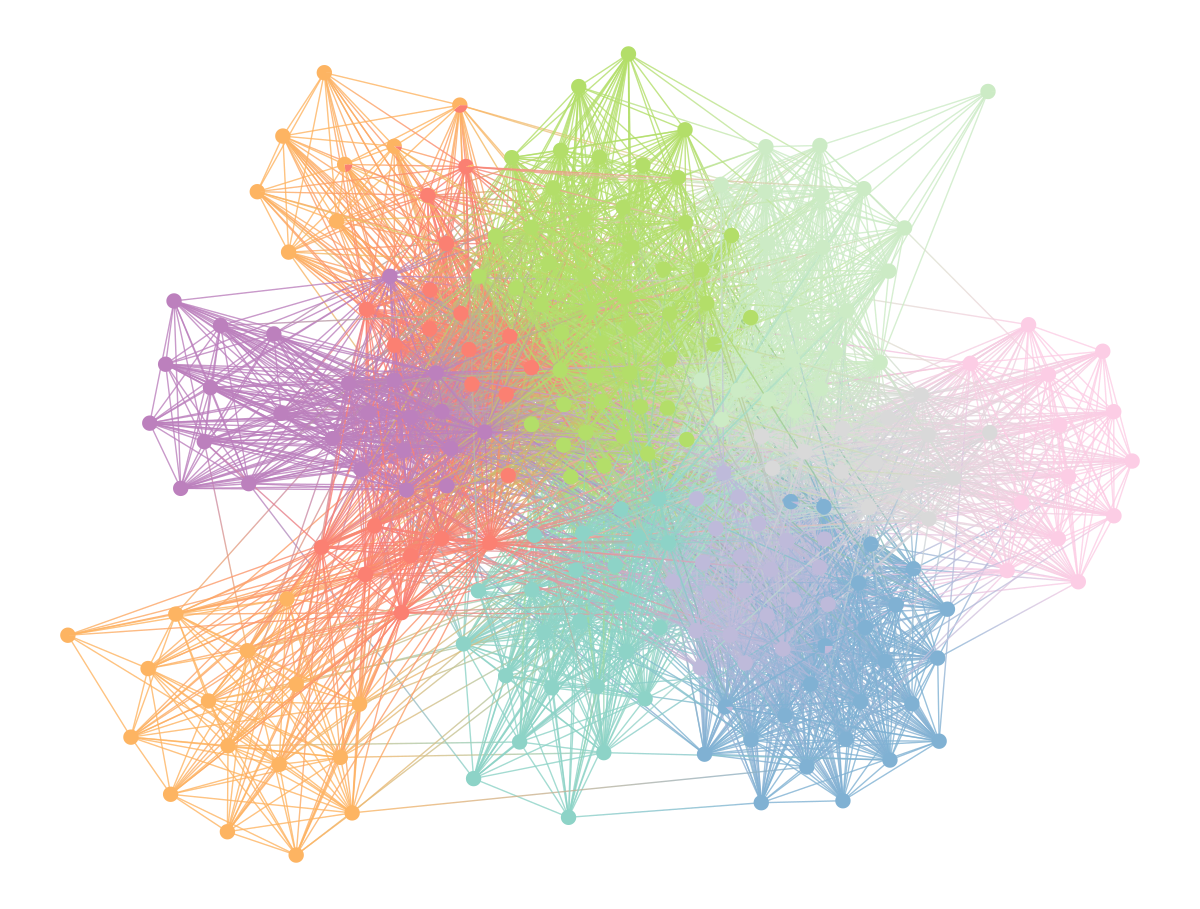
\includegraphics[width=\linewidth]{school-graph.png}
		\fbox{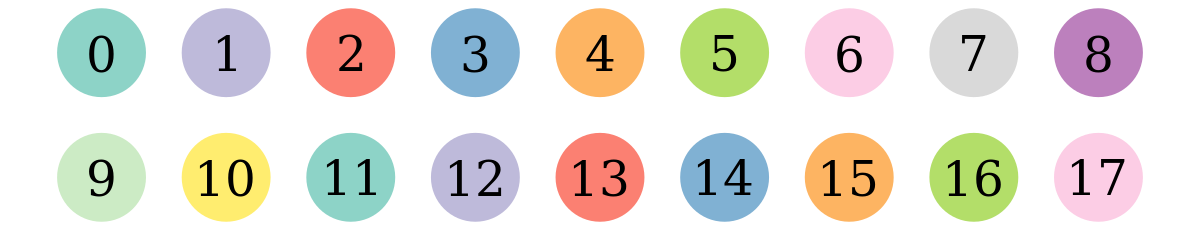
\includegraphics[width=0.5\linewidth]{school-legend.png}}
		\caption{Graph coloured by inferred block memberships of each node}
		\label{fig:school-graph}
	\end{subfigure}
	\hfill
	\begin{subfigure}{0.45\linewidth}
		\centering
		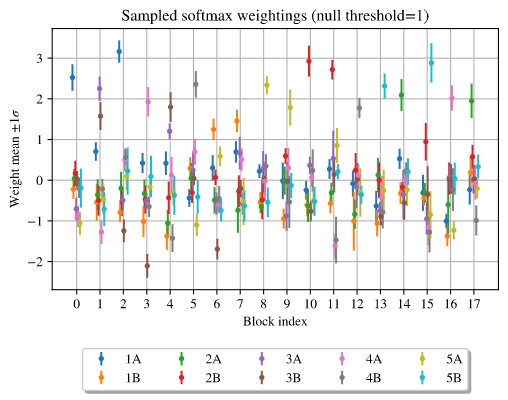
\includegraphics[width=\linewidth]{school-null.png}
		\caption{Feature-to-block generator sampled weight parameters for each block index}
		\label{fig:school-null}
	\end{subfigure}
	\caption{Primary school dynamic contacts network \cite{schools}}
\end{figure}
